\section{Some Python Results}



\begin{figure}
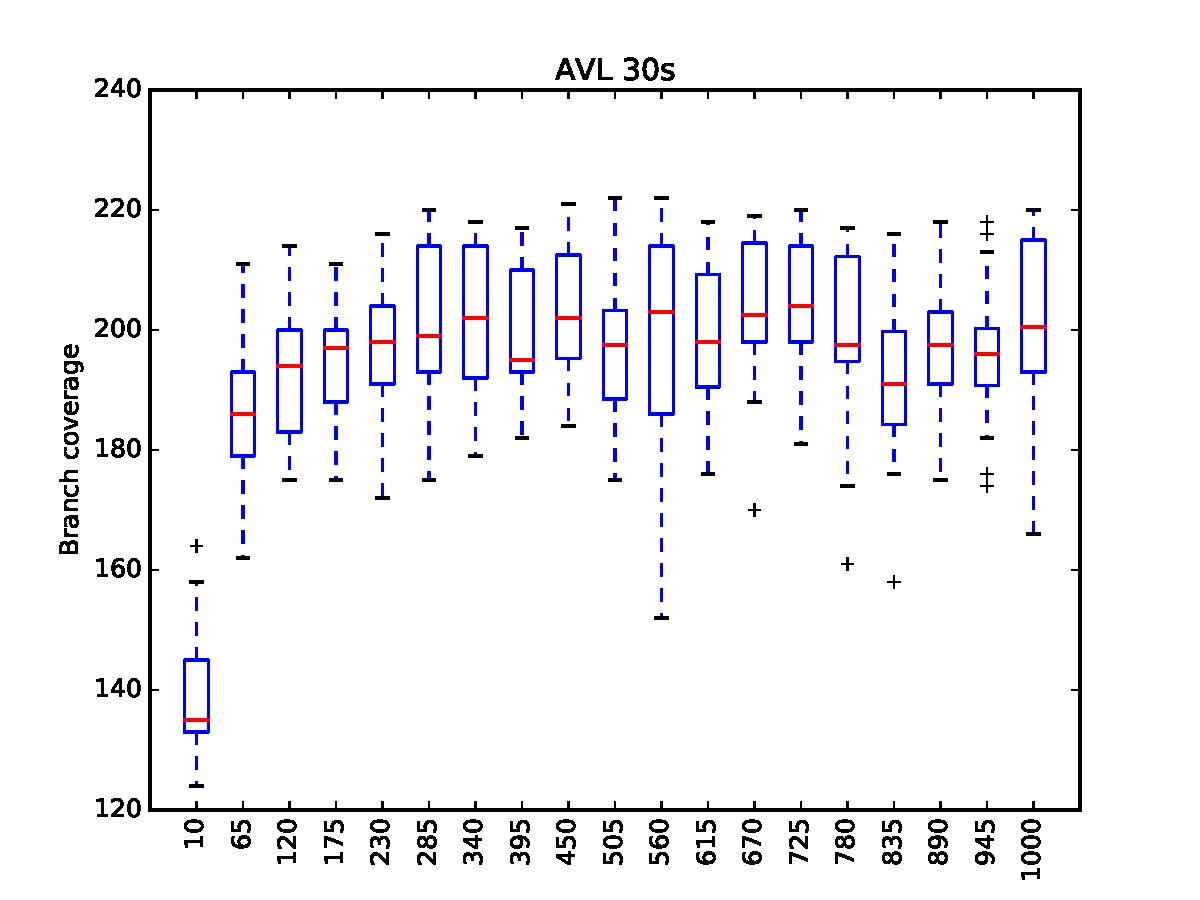
\includegraphics[width=\columnwidth]{graphs/AVLrand30}
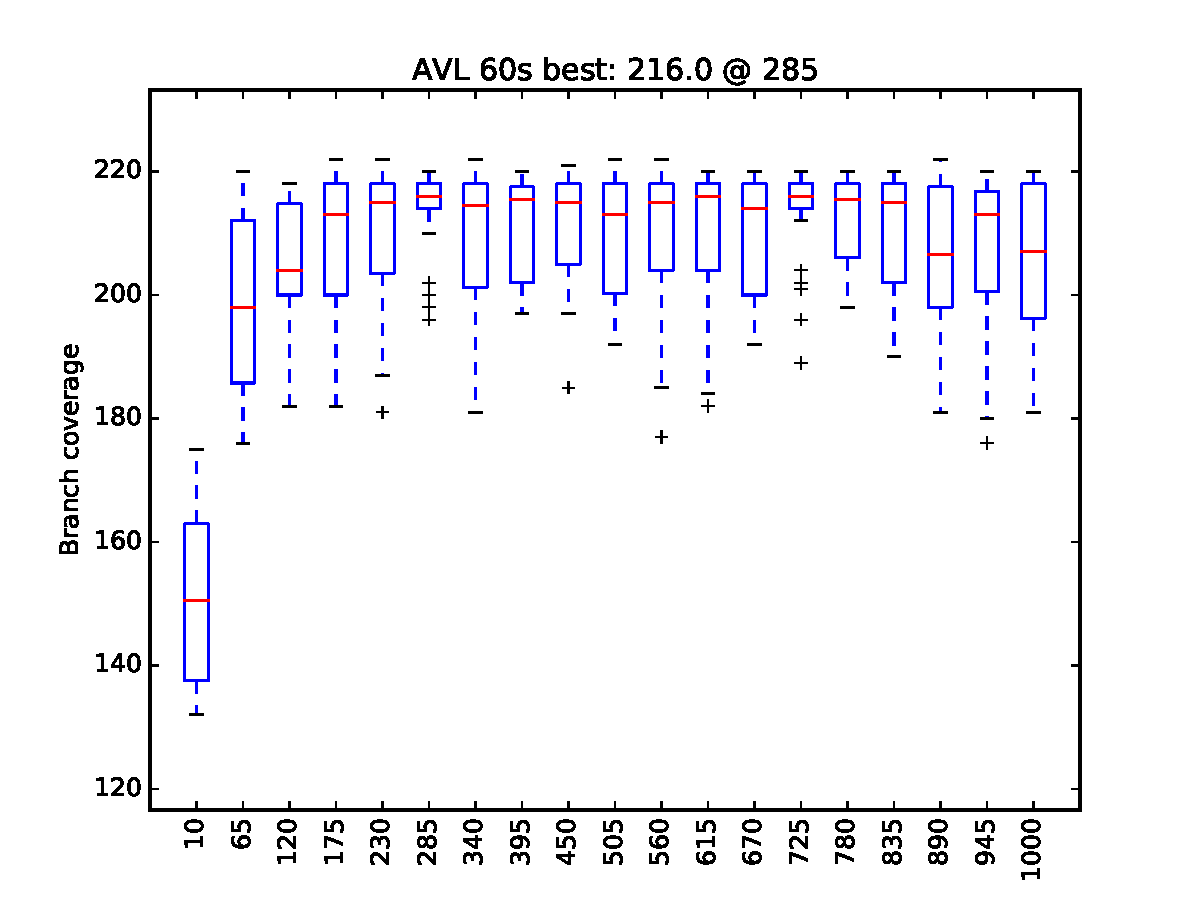
\includegraphics[width=\columnwidth]{graphs/AVLrand60}
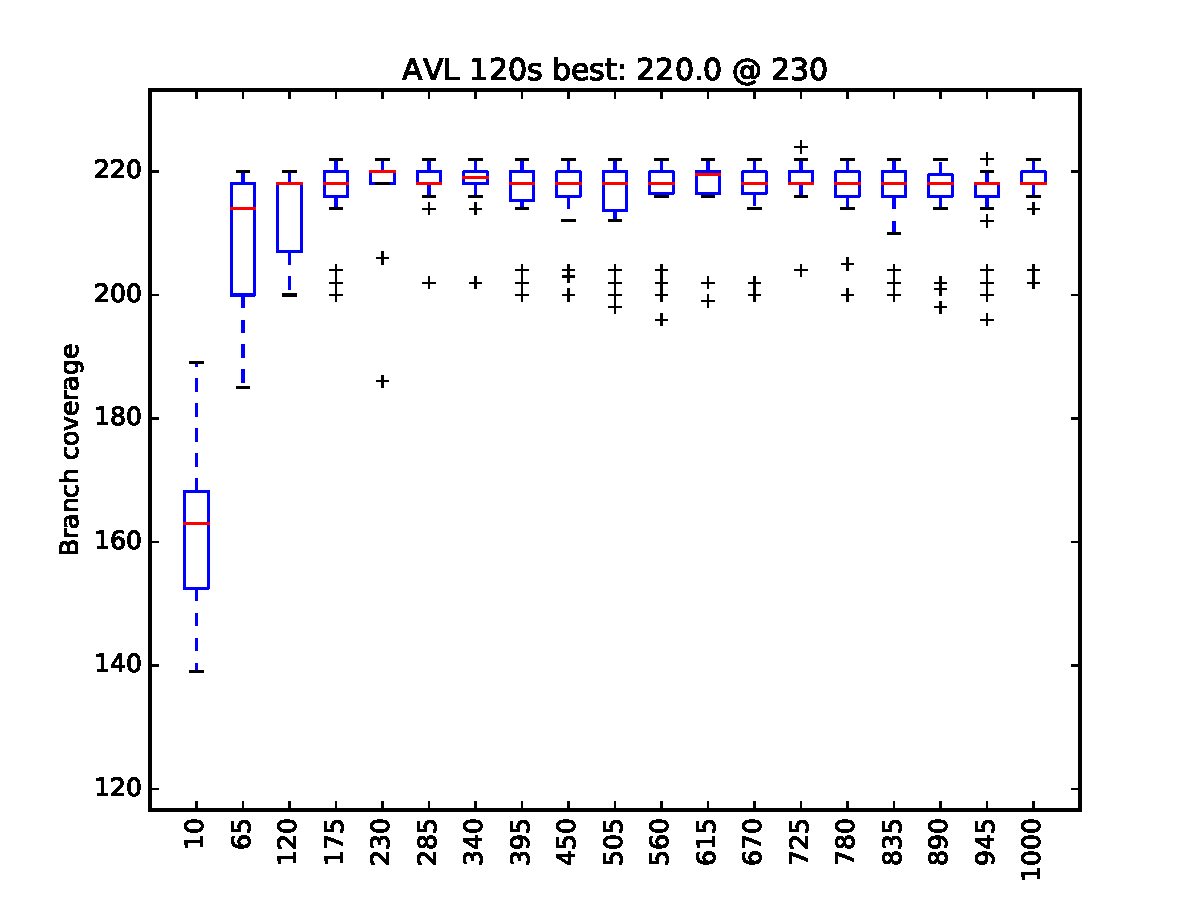
\includegraphics[width=\columnwidth]{graphs/AVLrand120}
\end{figure}

\begin{figure}
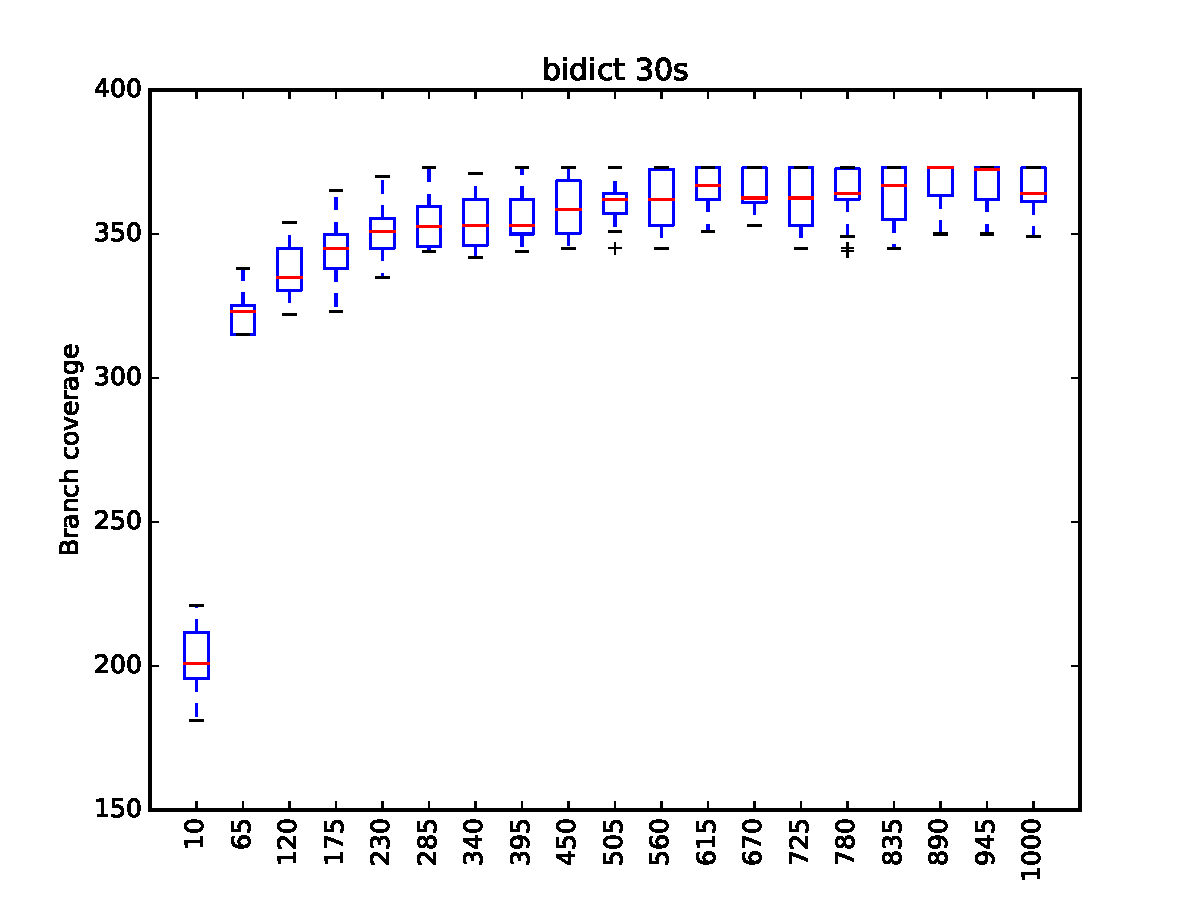
\includegraphics[width=\columnwidth]{graphs/bidictrand30}
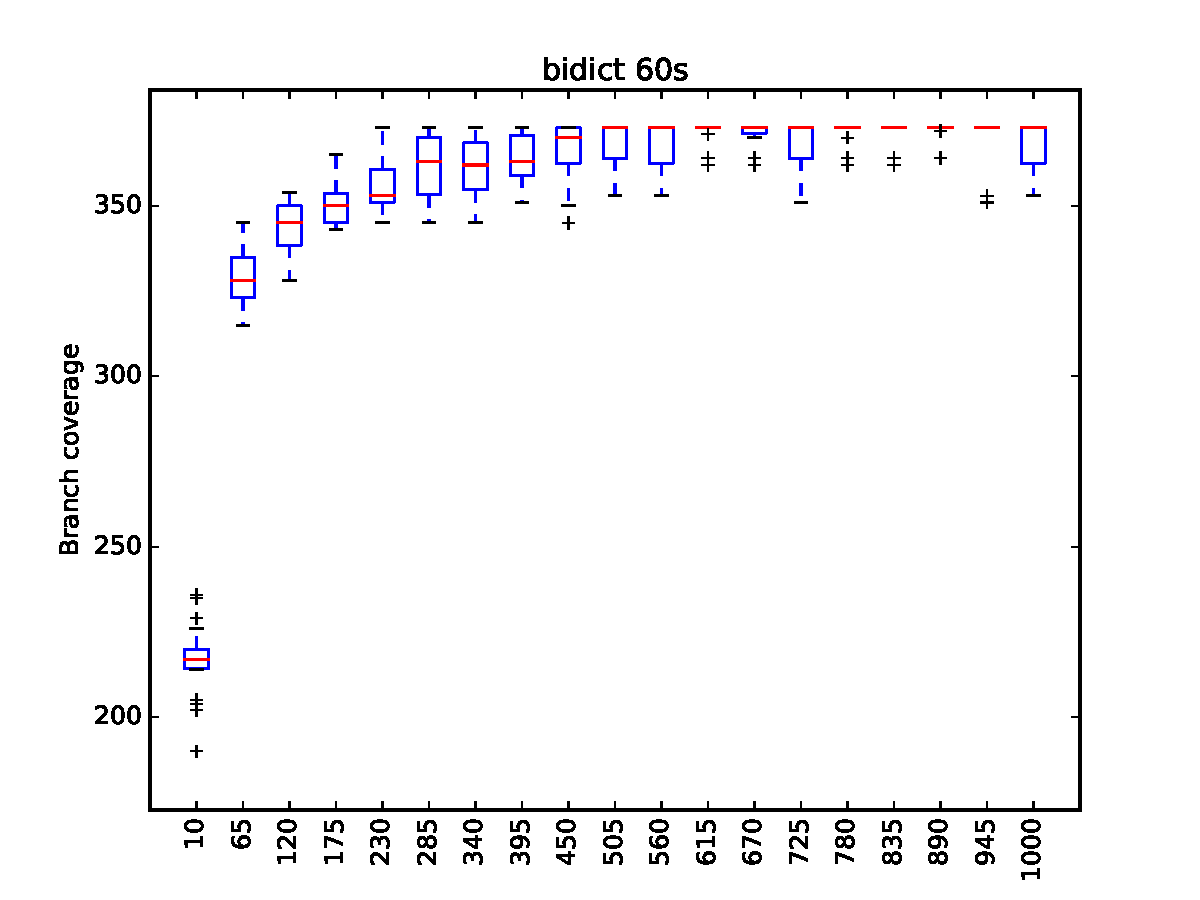
\includegraphics[width=\columnwidth]{graphs/bidictrand60}
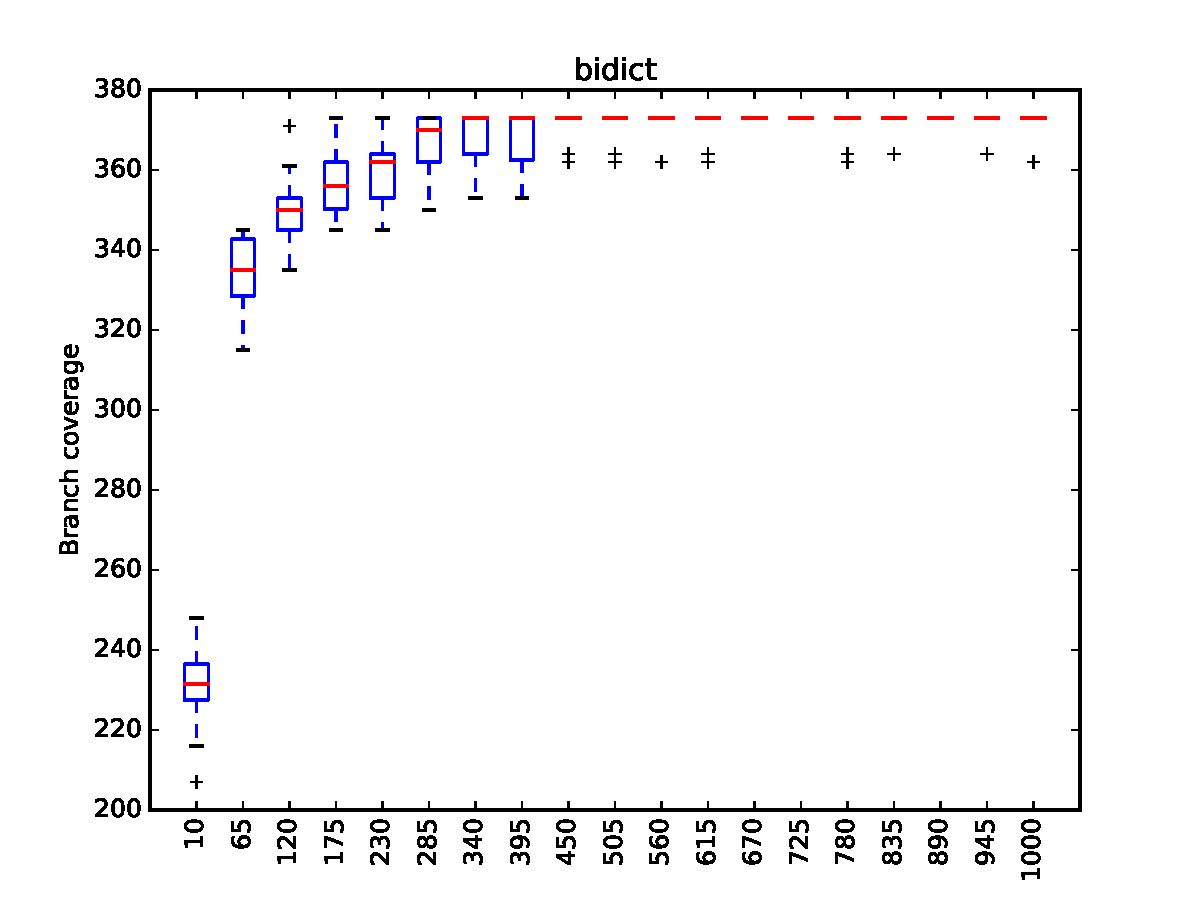
\includegraphics[width=\columnwidth]{graphs/bidictrand120}
\end{figure}


\begin{figure}
\includegraphics[width=\columnwidth]{graphs/Crand30}
\includegraphics[width=\columnwidth]{graphs/Crand60}
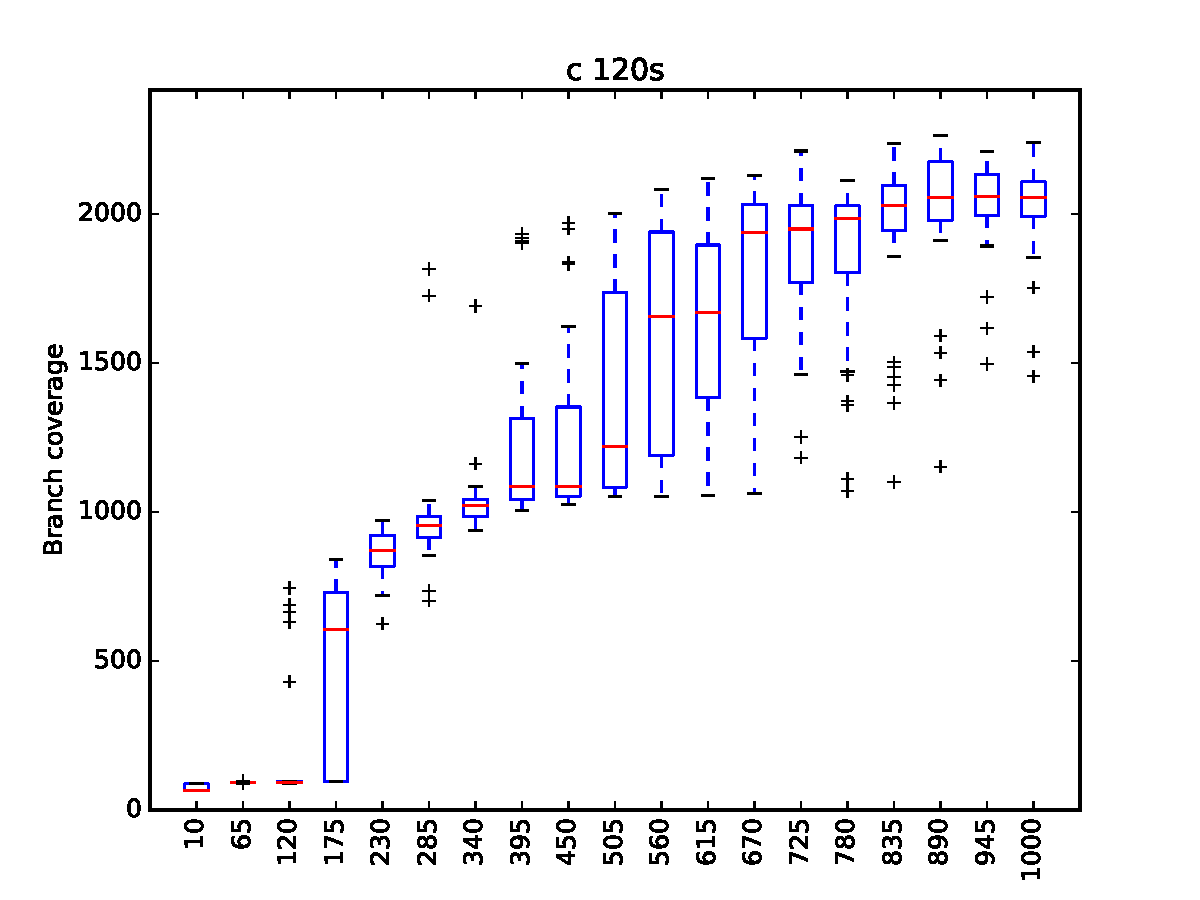
\includegraphics[width=\columnwidth]{graphs/Crand120}
\end{figure}


\begin{figure}
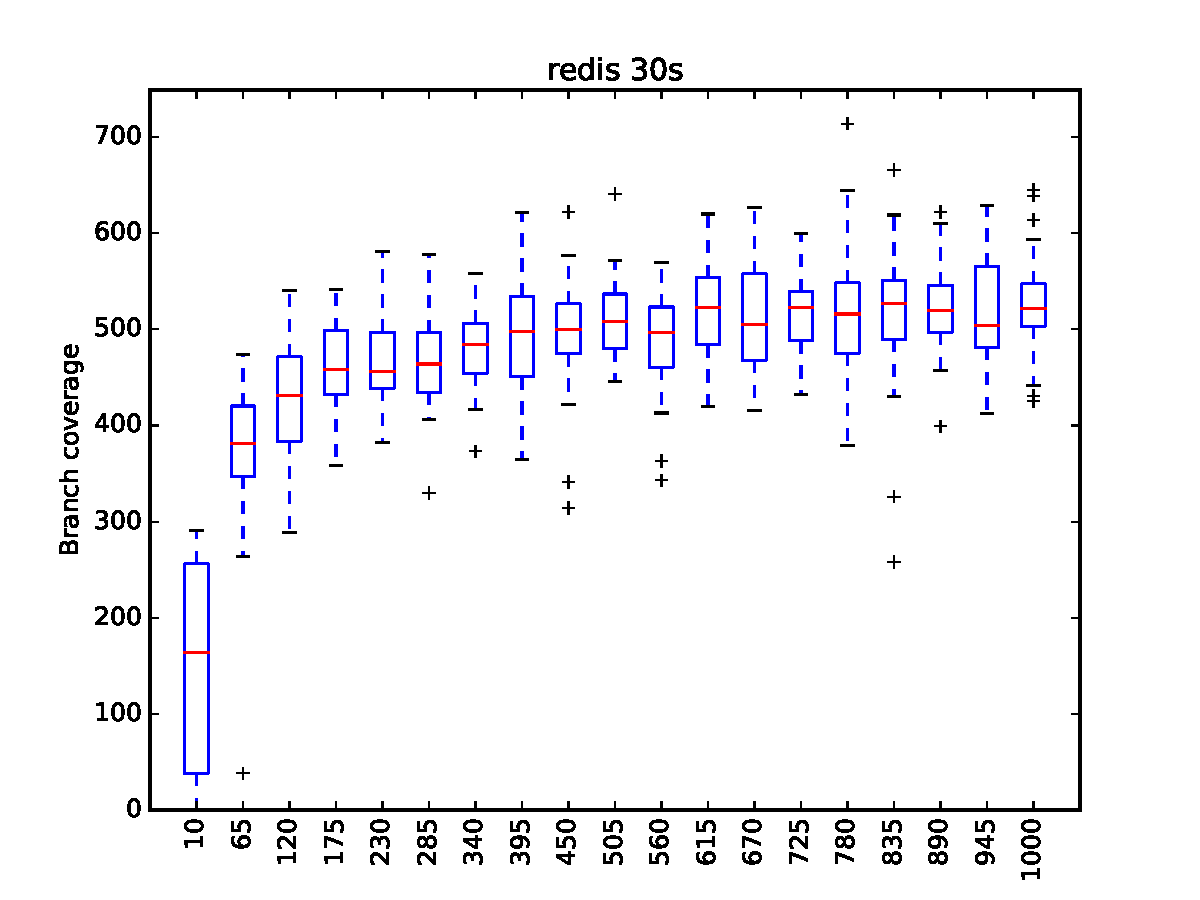
\includegraphics[width=\columnwidth]{graphs/redisrand30}
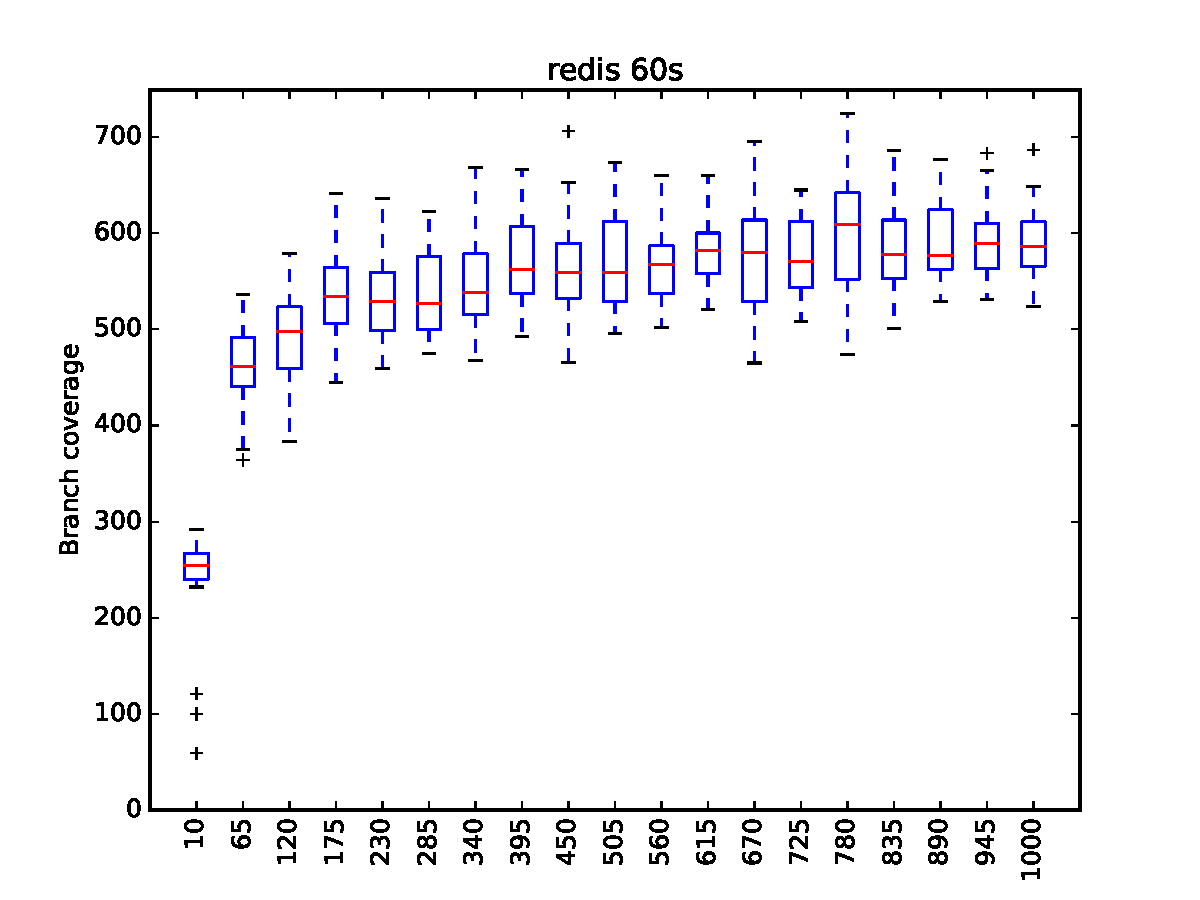
\includegraphics[width=\columnwidth]{graphs/redisrand60}
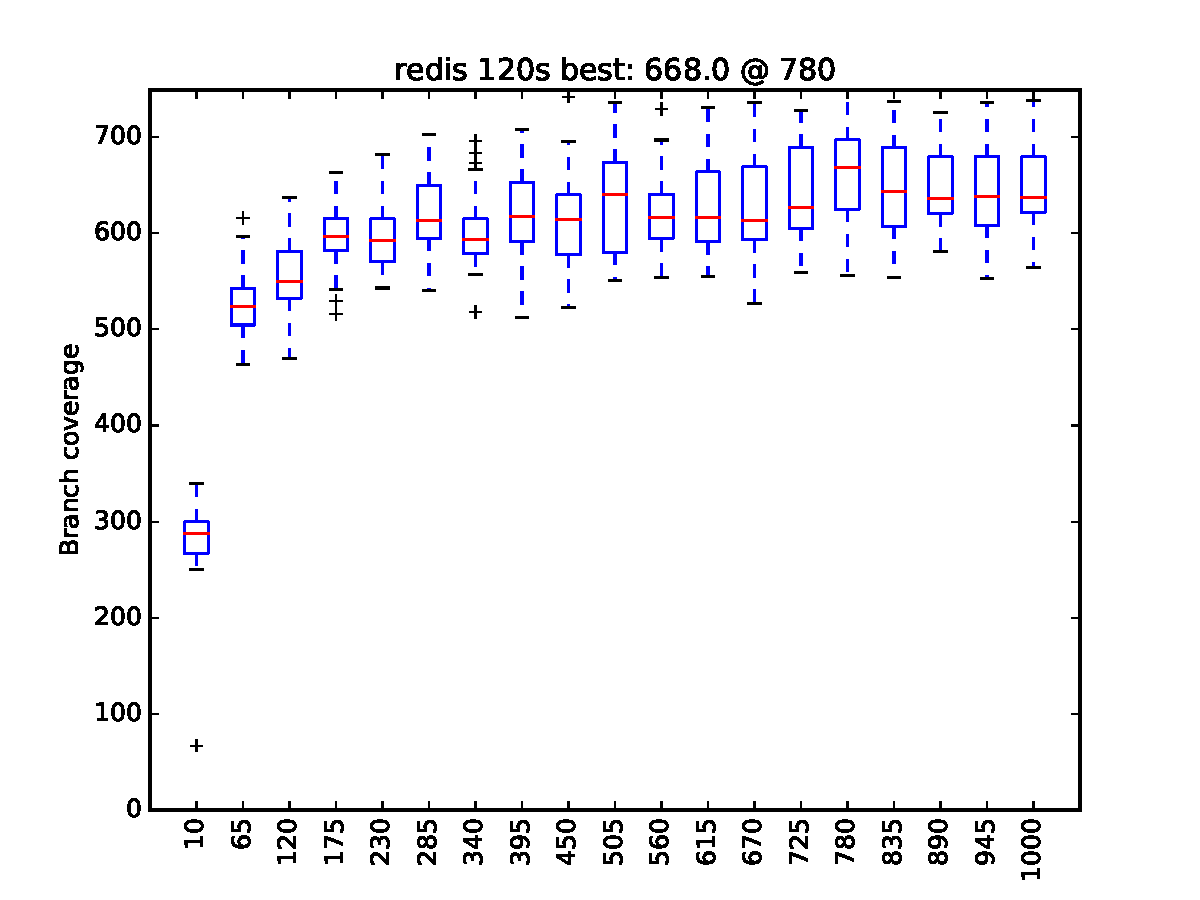
\includegraphics[width=\columnwidth]{graphs/redisrand120}
\end{figure}

\begin{figure}
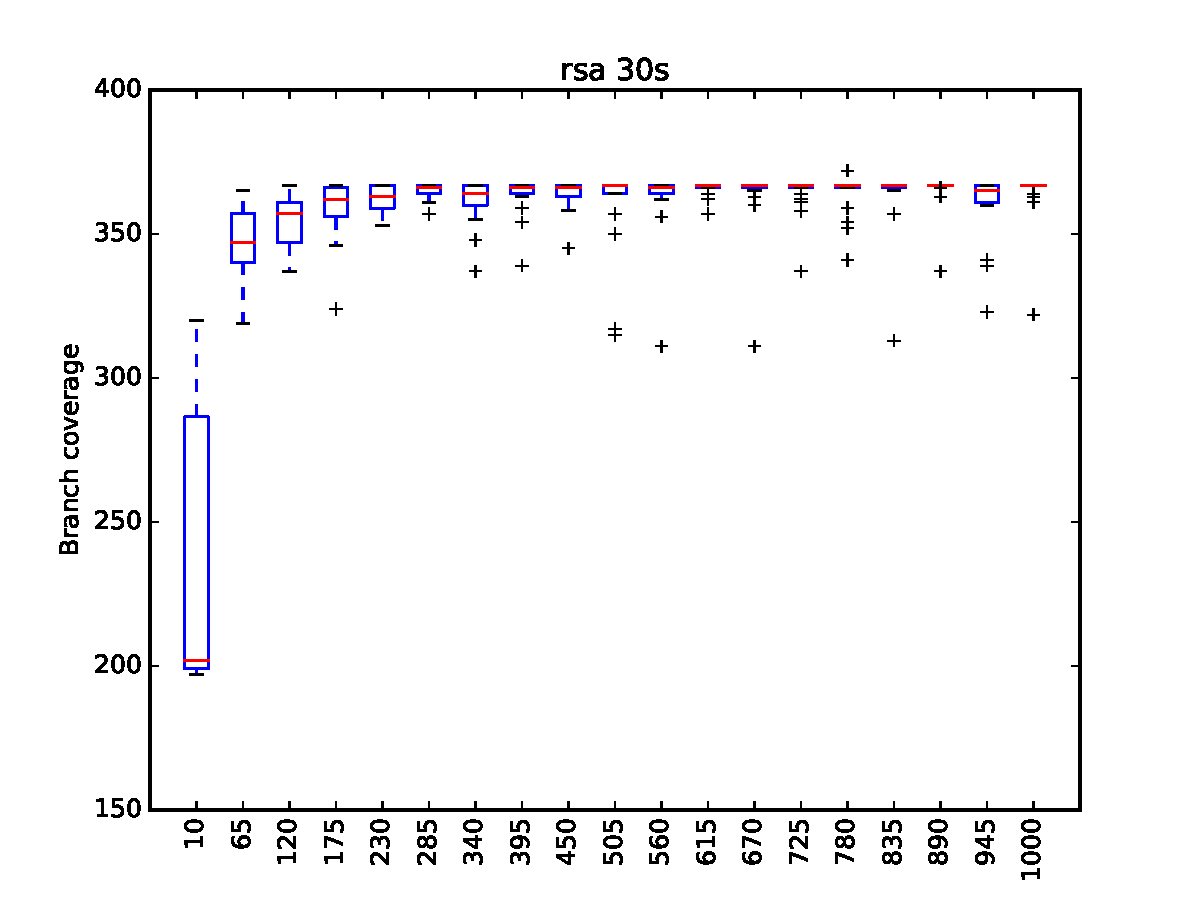
\includegraphics[width=\columnwidth]{graphs/rsarand30}
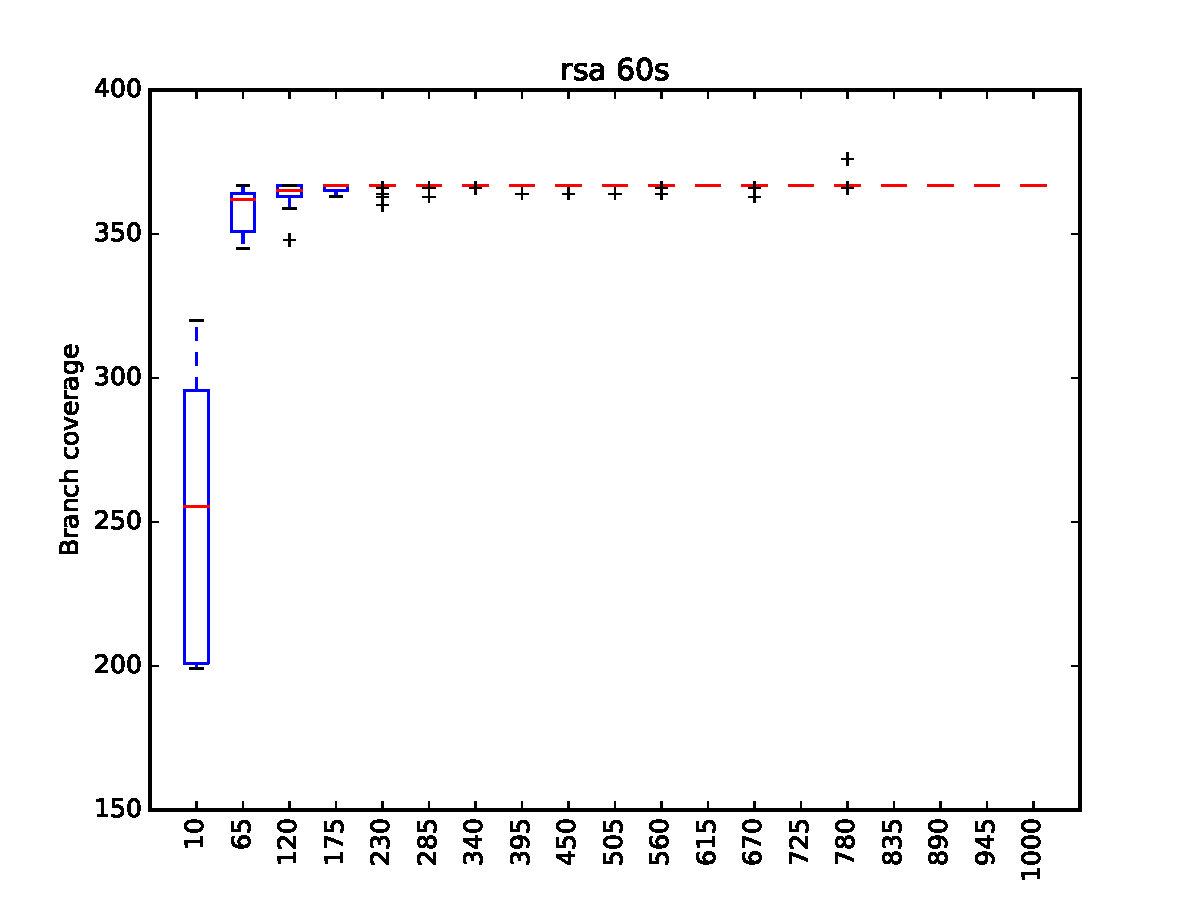
\includegraphics[width=\columnwidth]{graphs/rsarand60}
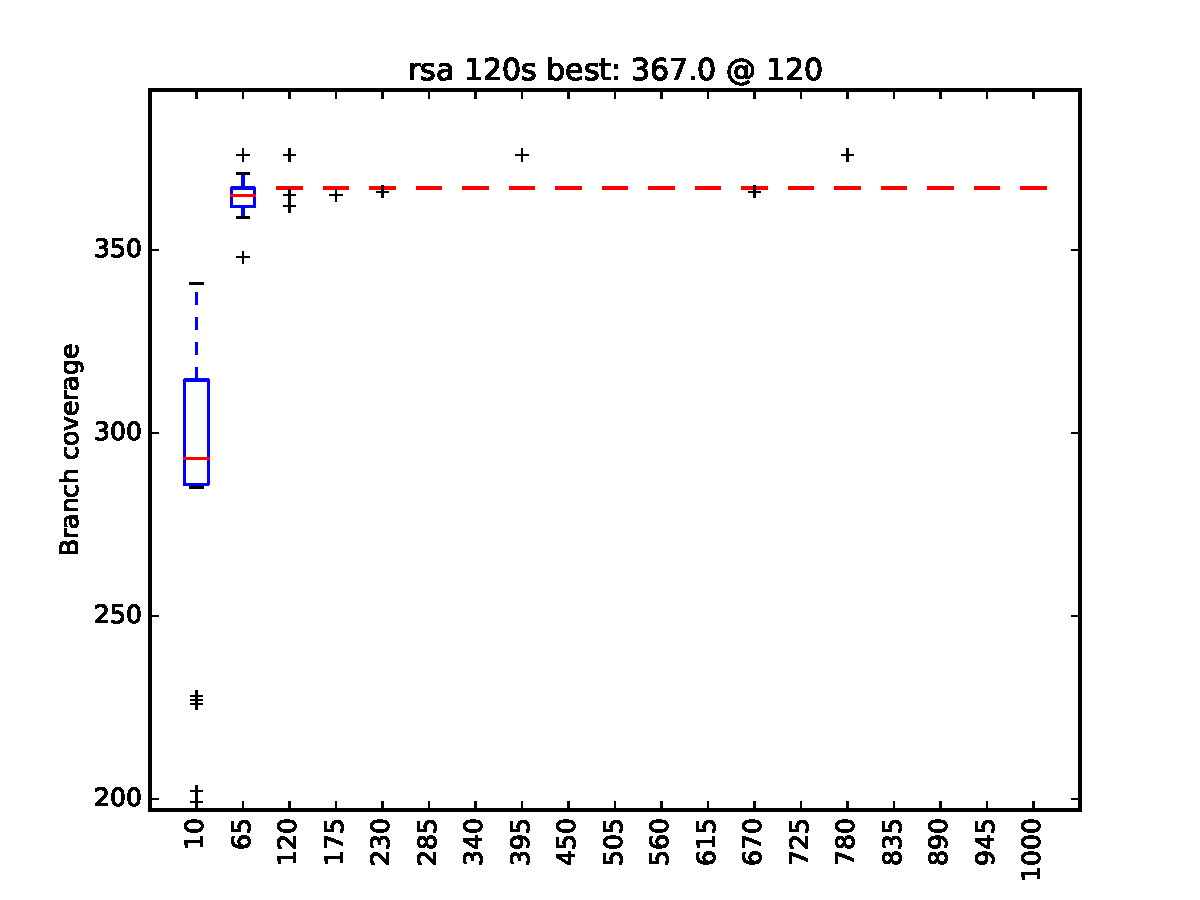
\includegraphics[width=\columnwidth]{graphs/rsarand120}
\end{figure}


\begin{figure}
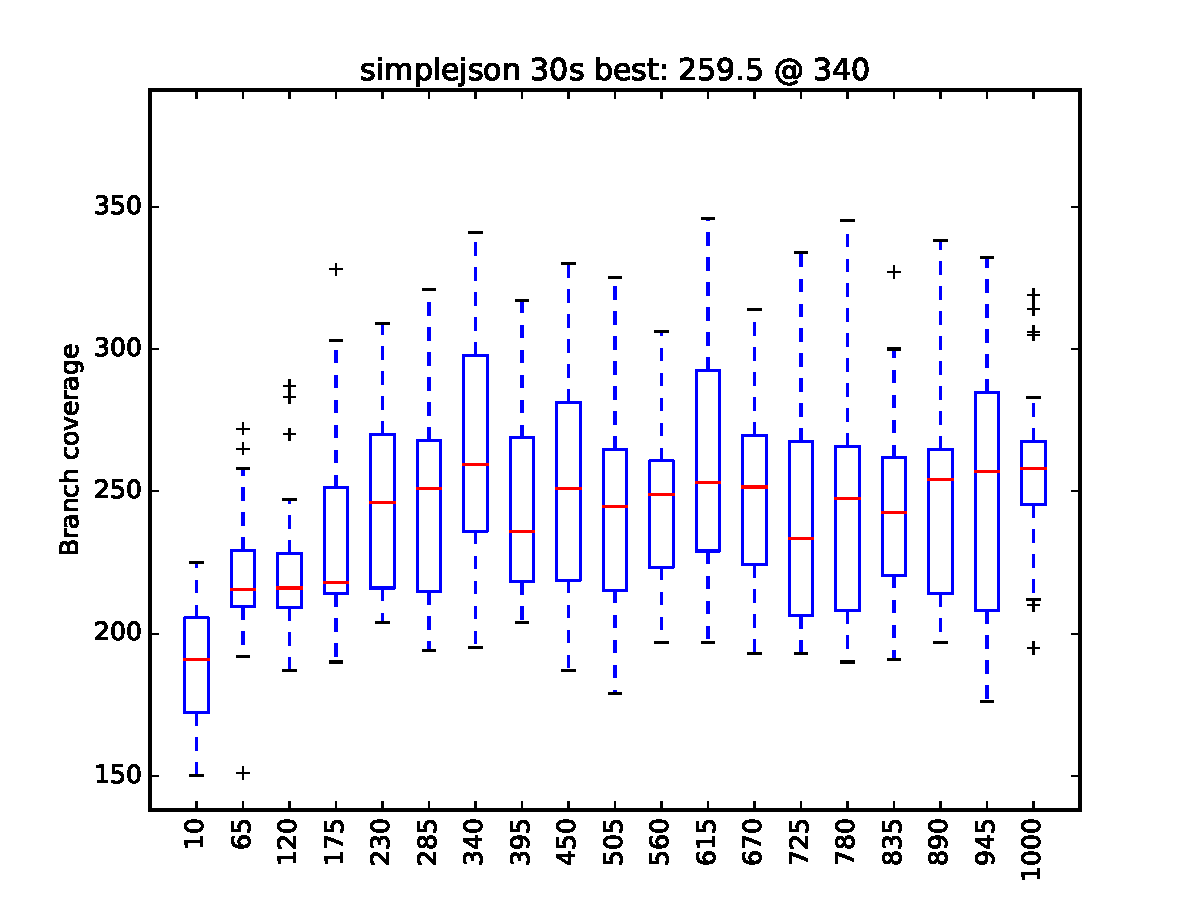
\includegraphics[width=\columnwidth]{graphs/simplejsonrand30}
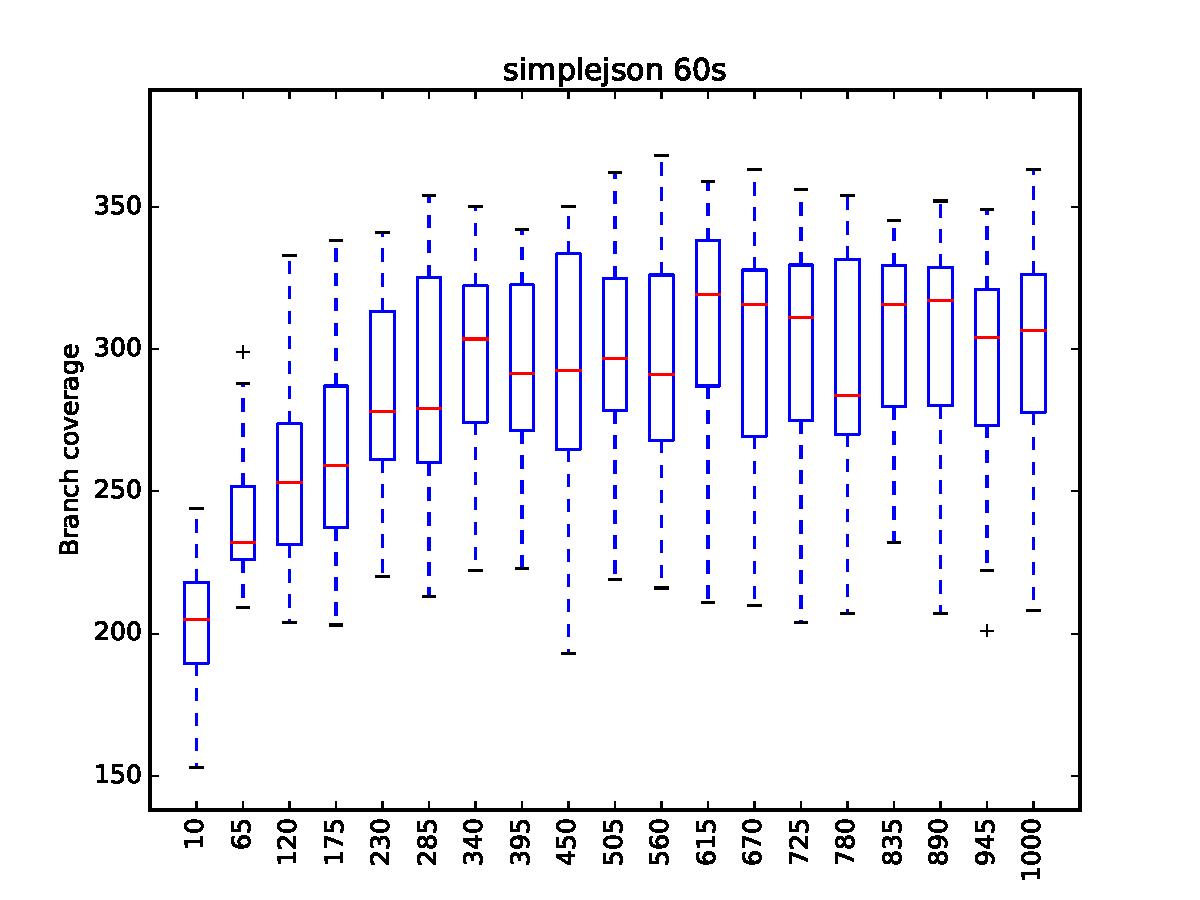
\includegraphics[width=\columnwidth]{graphs/simplejsonrand60}
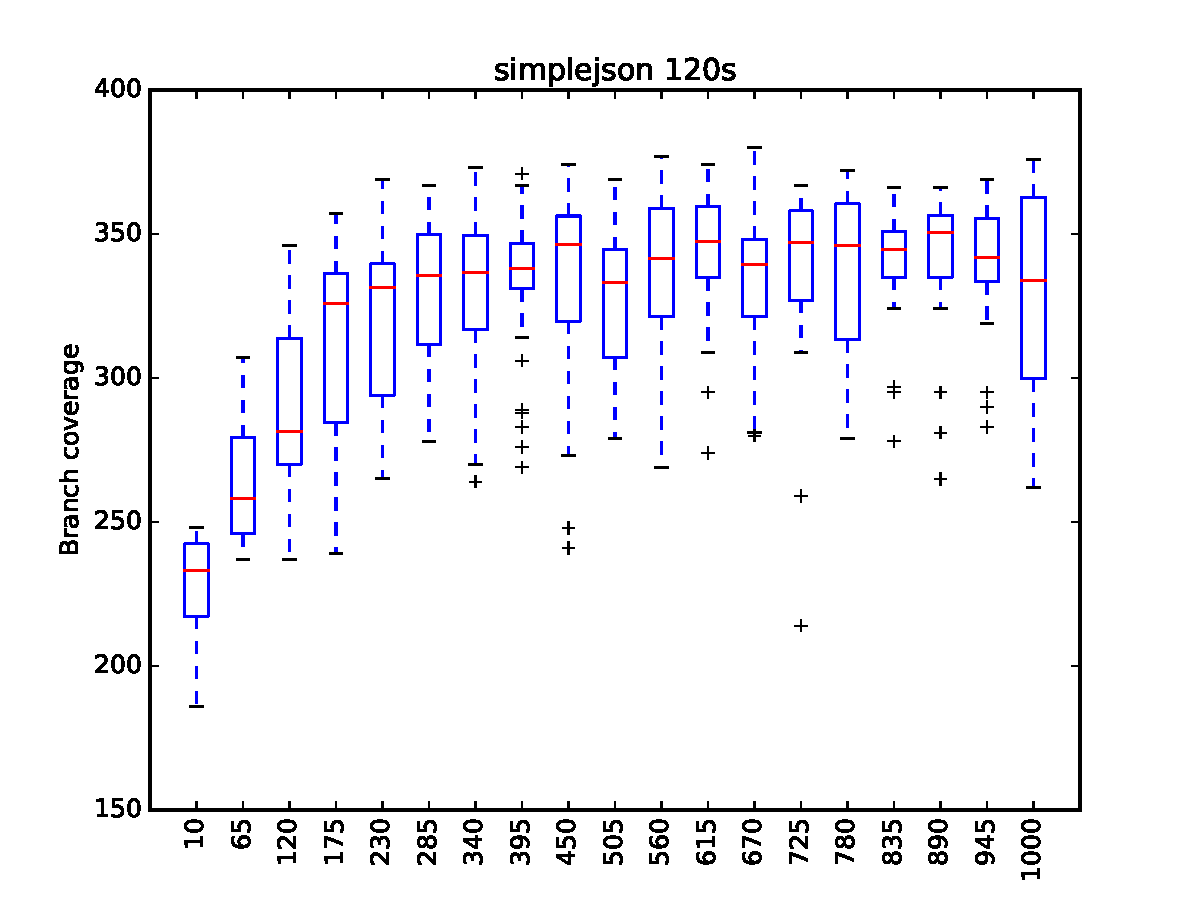
\includegraphics[width=\columnwidth]{graphs/simplejsonrand120}
\end{figure}

\begin{figure}
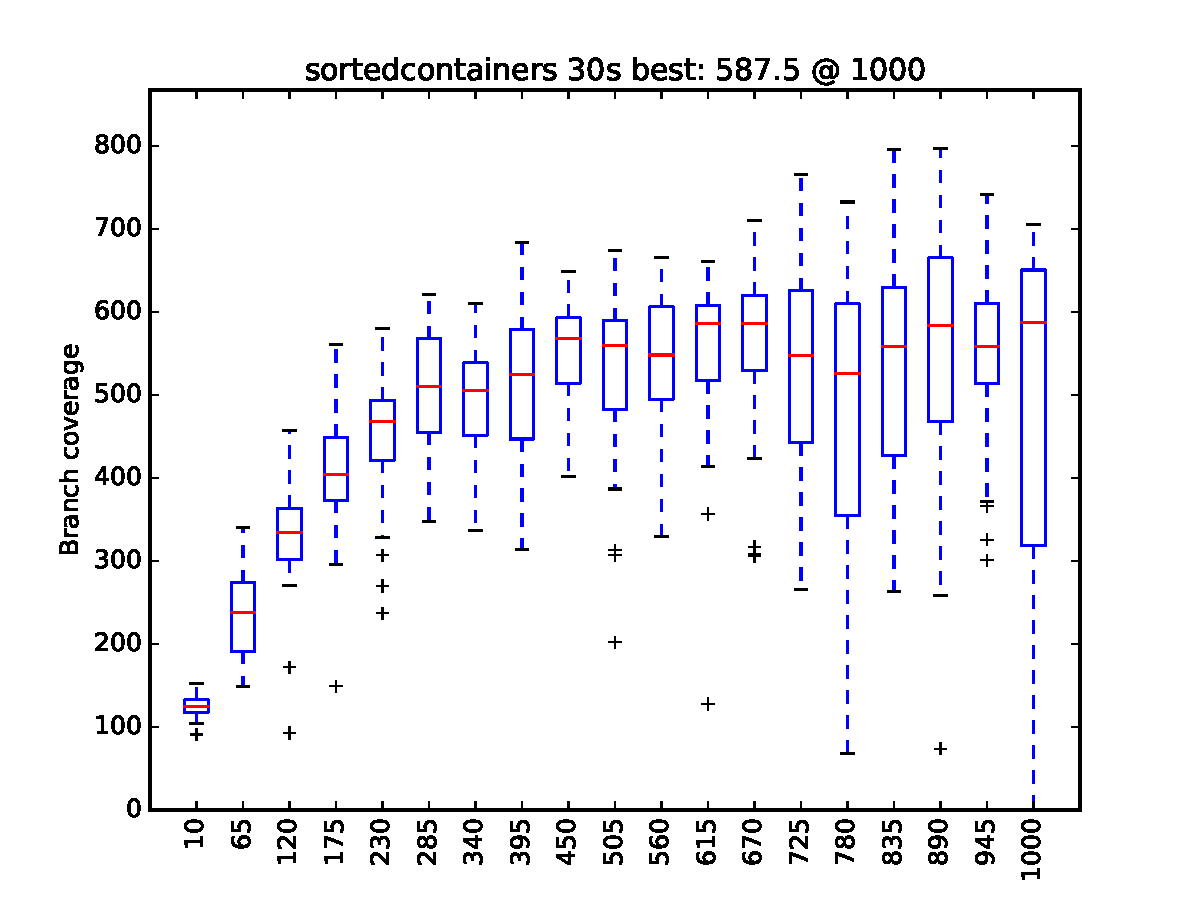
\includegraphics[width=\columnwidth]{graphs/sortedcontainersrand30}
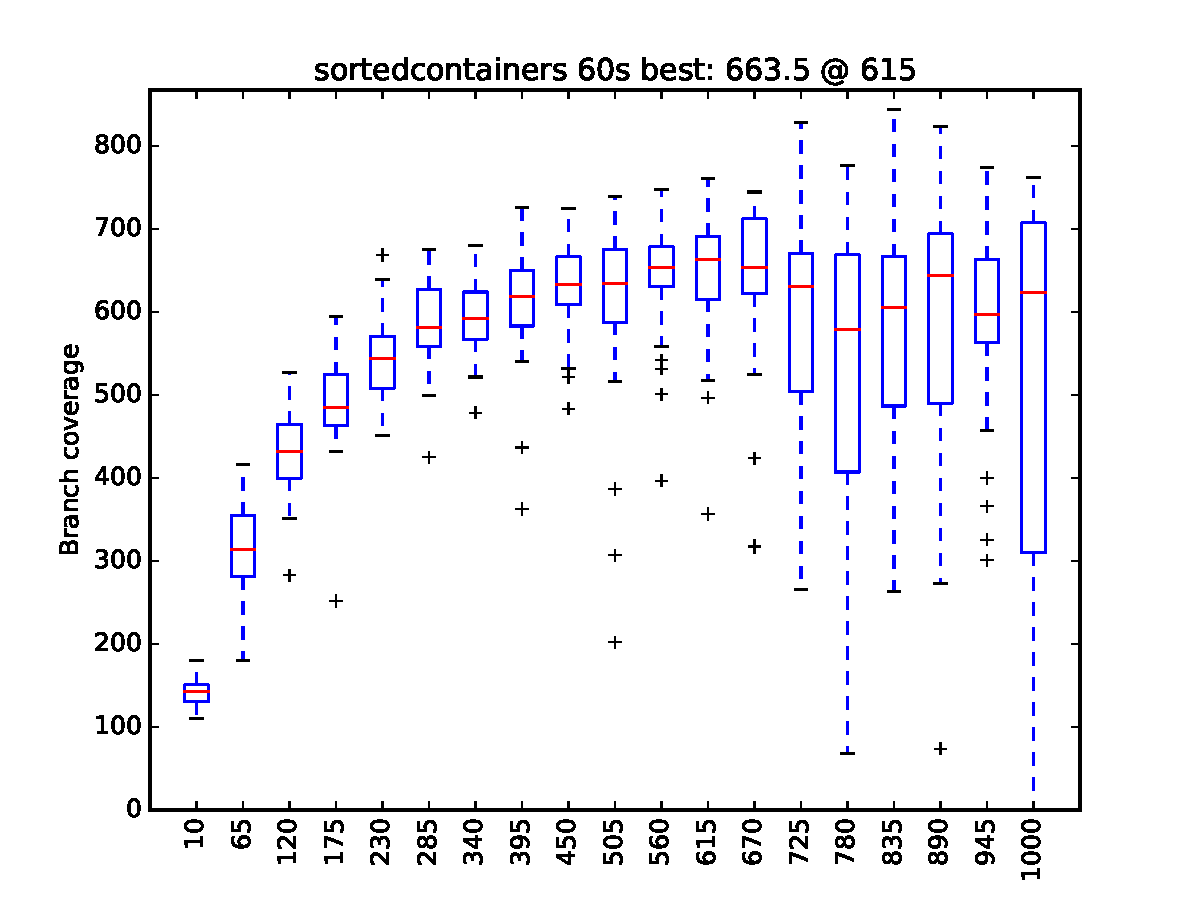
\includegraphics[width=\columnwidth]{graphs/sortedcontainersrand60}
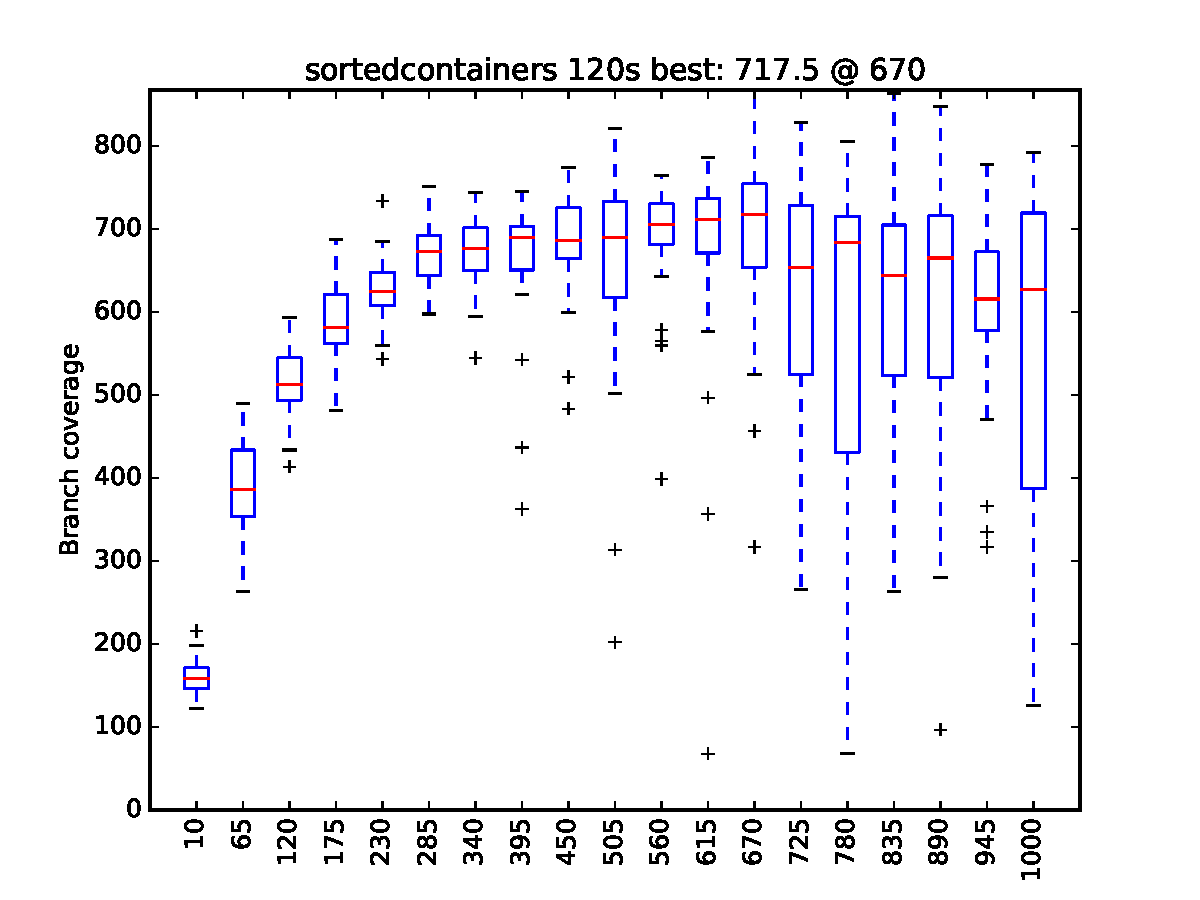
\includegraphics[width=\columnwidth]{graphs/sortedcontainersrand120}
\end{figure}

\begin{figure}
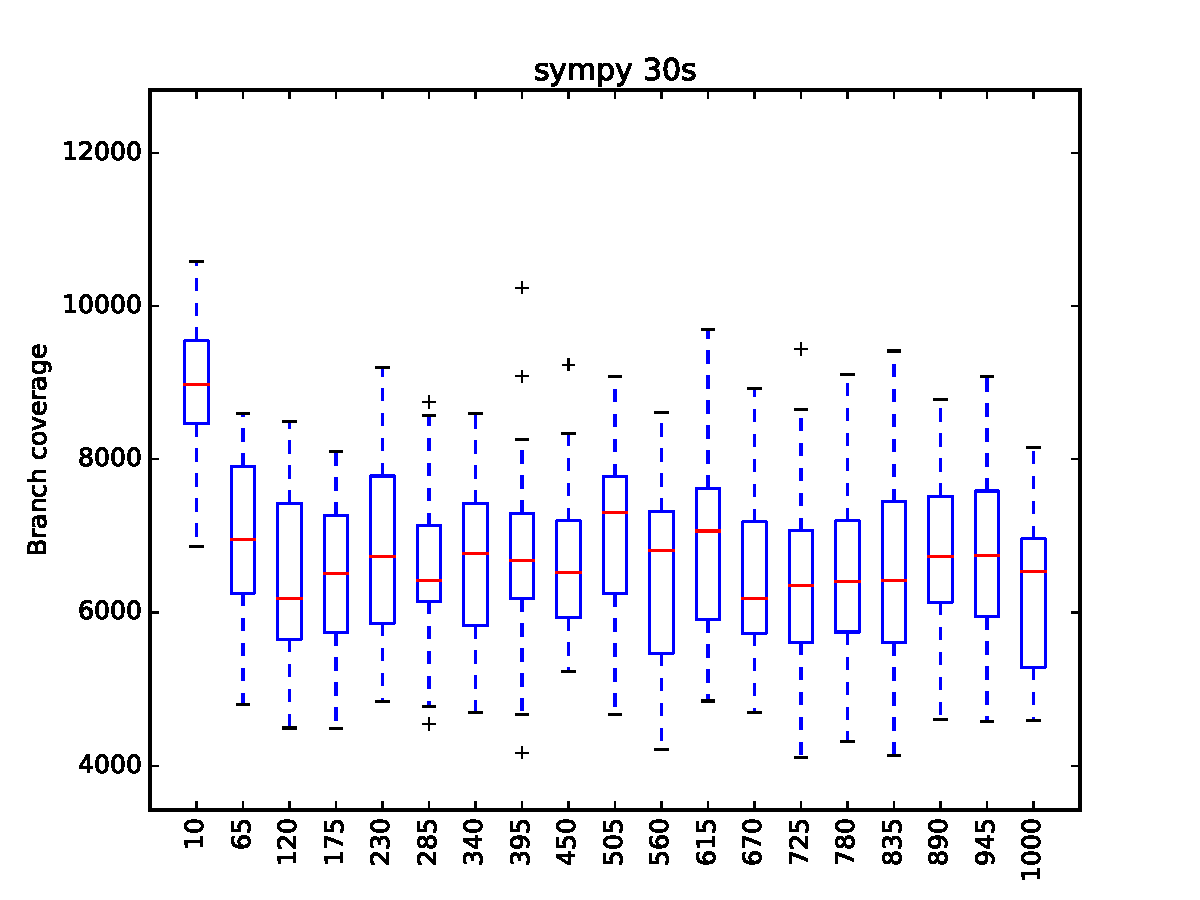
\includegraphics[width=\columnwidth]{graphs/sympyrand30}
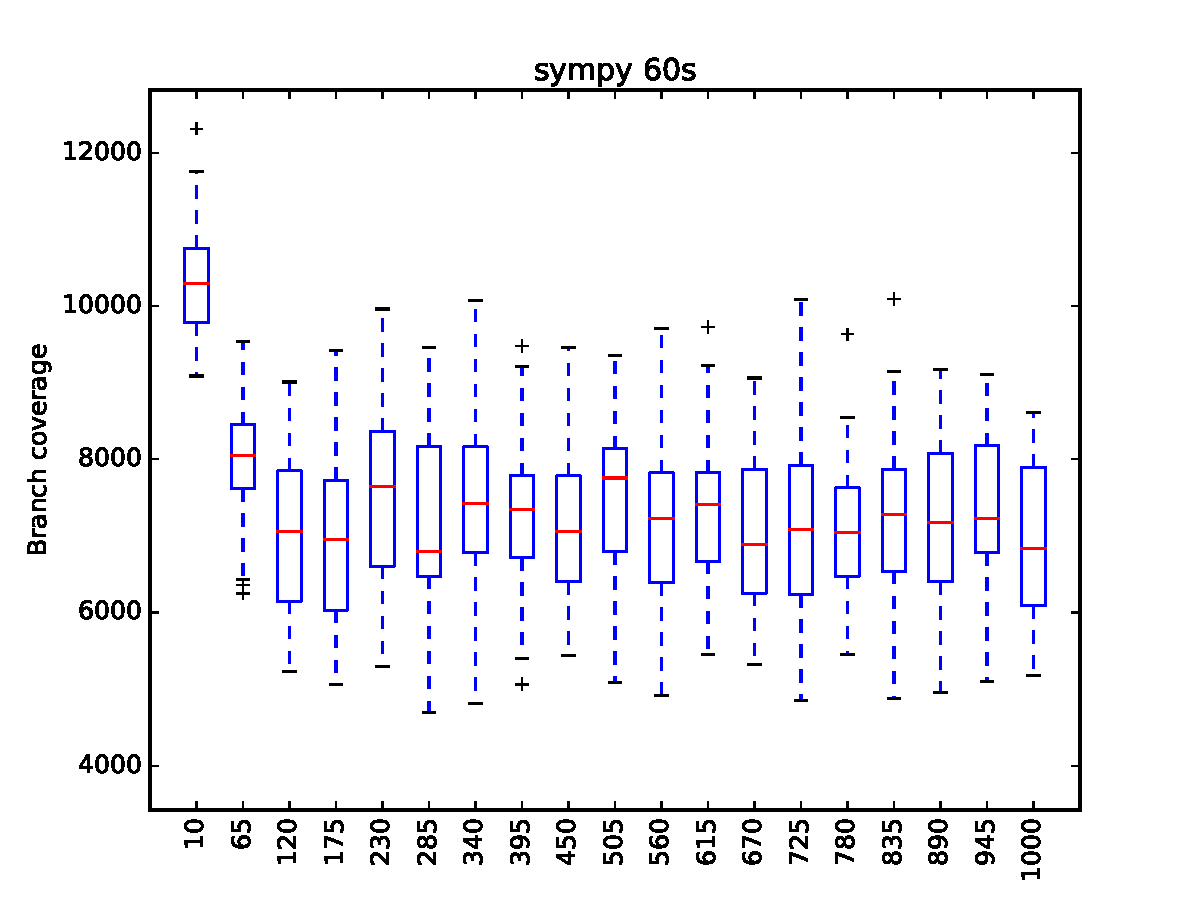
\includegraphics[width=\columnwidth]{graphs/sympyrand60}
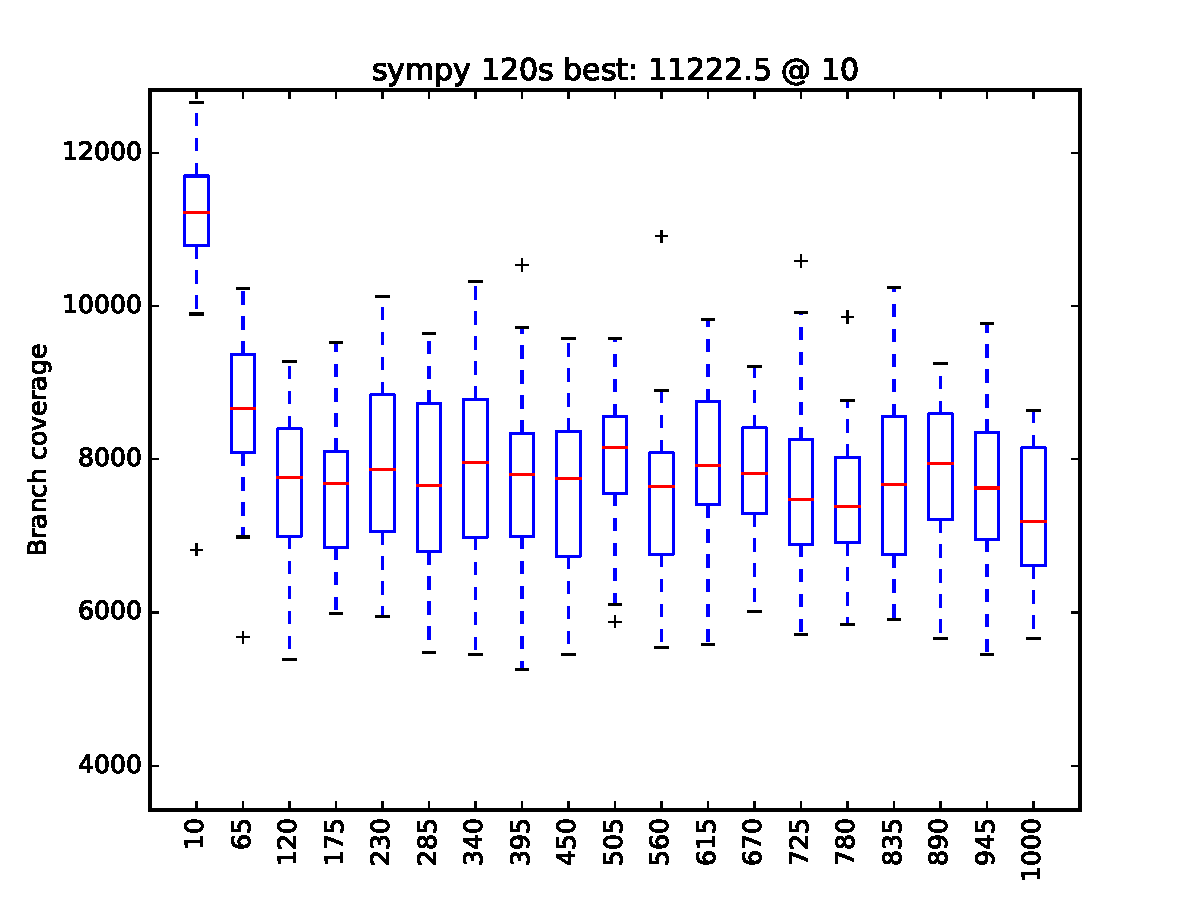
\includegraphics[width=\columnwidth]{graphs/sympyrand120}
\end{figure}
